\chapter{Methodological Approach}
\textcite[22-23]{Pohl.2007} explains, that applied requirements engineering must always be closely connected to the architectural planning. This is because the architecture of a application induces insights, which can either lead to conflicts, or to gaps in the requirements set at the give state of work \parencites[22-23]{Pohl.2007}. \Cref{fig:iterative} shows that with an increase in the level of detail, a repeating comparison of the problem (requirement) and solution (concept) perspective to check the impacts on realization.

\begin{figure}[H]
    \centering
    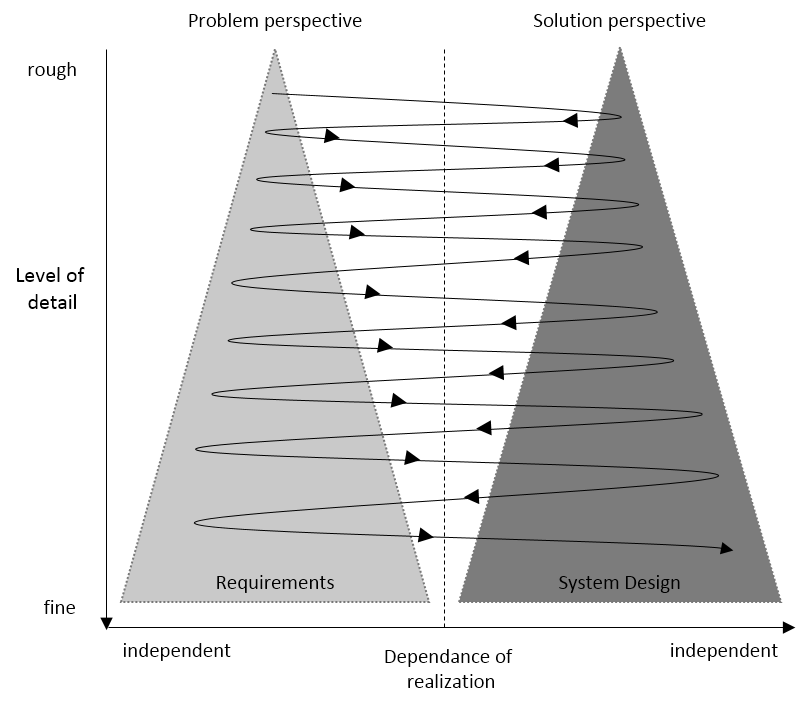
\includegraphics[width=0.7\textwidth]{img/iterative.png}
    \caption[Interdependence of Requirements and Design]{Interdependence of Requirements and Design \parencite[23]{Pohl.2007}}
    \label{fig:iterative}
\end{figure}

\paragraph{} This reflects the iterative nature of requirements engineering as described on \cpageref{iterative}. Thereby a check for bidirectional implications of architecture concept and requirement will be made by the end of the following procedure.

\paragraph{} The practical appliance will start with the definition of the context and then continue with the performance of the three main activities (cf. \cpageref{mainactivity} and \cpagerefrange{beginmain}{endmain}). An Architectural concept will be created, as described above, followed by a visual concept. 


\section{Finding the Context Definition}
This thesis will start the requirement engineering as suggested by \textcite[55]{Pohl.2007} and described in \cref{ssec:reqEn} by available input information. This paper will orientate at the source categories shown in \Cref{fig:reqFlow} on \cpageref{fig:reqFlow} going top down. 

\paragraph{} In the first instance, a sketch system context diagram will be created. Secondly, personas (cf. \Cref{ssec:personas}) will be produced, in order to get an idea of the stakeholders. Concluding from the personas and other sources of information, goals will identified. These will be analyzed for implications on the facets of the system context, as described on \cpagerefrange{beginFacets}{endFacet}.


\subsection{System Context Diagram}
\begin{figure}[H]
    \centering
    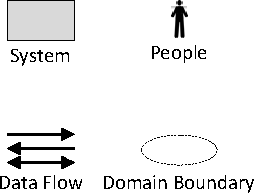
\includegraphics[scale=1]{img/SCDSymbols.pdf}
    \caption[Symbols of System Context Diagrams]{Symbols of System Context Diagrams \parencites[77]{Lauesen.2008}}
    \label{fig:scdSym}
\end{figure}
The system context diagram consists of four components: system, people, data flow, and domain boundaries \parencites[cf.][76-77]{Lauesen.2008}. Each one has its own representation, displayed in \Cref{fig:scdSym}. System context diagrams are used to identify required interfaces \parencites[cf.][75]{Lauesen.2008}, as well as to define the system boundary \parencites[cf.][75]{Ebert.2014}. It is an important overview of requirement sources, reflecting all interacting systems and persons. The direction of the arrow can show the direction of the data flow, or more commonly display the direction of intend \parencite[cf.][77]{Lauesen.2008}. In this paper the direction of an arrow will display the direction of intend.

\begin{figure}[H]
    \centering
    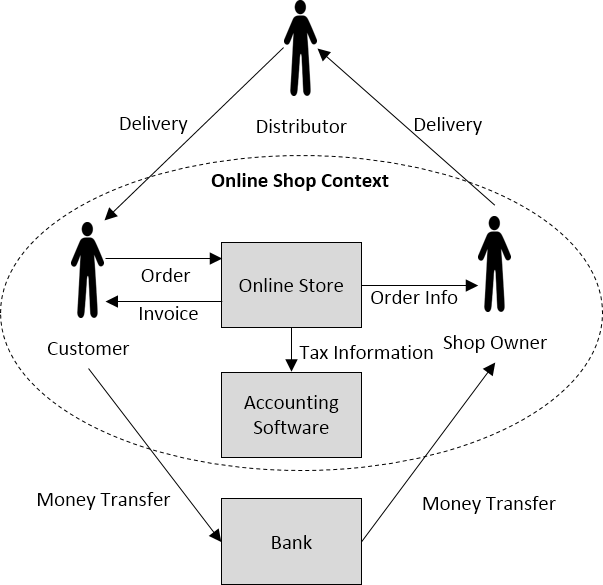
\includegraphics[height=.5\textheight]{img/SystemContextExample.png}
    \caption[System Context Diagram Example]{System Context Diagram Example (own illustration)}
    \label{fig:scEx}
\end{figure}

\Cref{fig:scEx} depicts an example of that a \ssay{Customer} shall be able to send an \ssay{Order} to the \ssay{Online Store}, which sends the \ssay{Order Info} to the \say{Shop Owner}, the \ssay{Tax Information} to the \ssay{Accounting Software} and the \ssay{Invoice} to the \ssay{Customer}. These interactions inside the \ssay{Online Shop Context} are regarded 'in scope', as opposed the \ssay{Distributor} and the \ssay{Bank}, which are regarded as out of scope.

\subsection{Personas \label{ssec:personas}}

Personas are representations of target groups as individual archetypal person \parencite[cf.][81]{Cooper.2007}. They have got all of the attributes a natural person, including a name, gender, age, family, education, and most importantly: a motivation \parencites[cf.][]{Platt.2016}[cf.][83-84]{Cooper.2007}. 

\paragraph{} Human brains care more bout individuals than large groups \parencite[cf.][]{Platt.2016}. Therefore, archetypal individual people \parencite[cf.][81-82]{Cooper.2007}, which embody specific characteristics of groups \parencite[cf.][]{Platt.2016} are more easy to understand and consider in the requirements engineering process.

\paragraph{} Identifying, analyzing, and prioritizing personas is always based on research \parencites[cf.][39]{Robier.2016}[cf.][80]{Cooper.2007}. Although these methods do not claim to be scientifically accurate, they must not be based upon stereotypes and arbitrary decisions \parencite[cf.][82-83]{Cooper.2007}. 

\begin{figure}[H]
\centering
    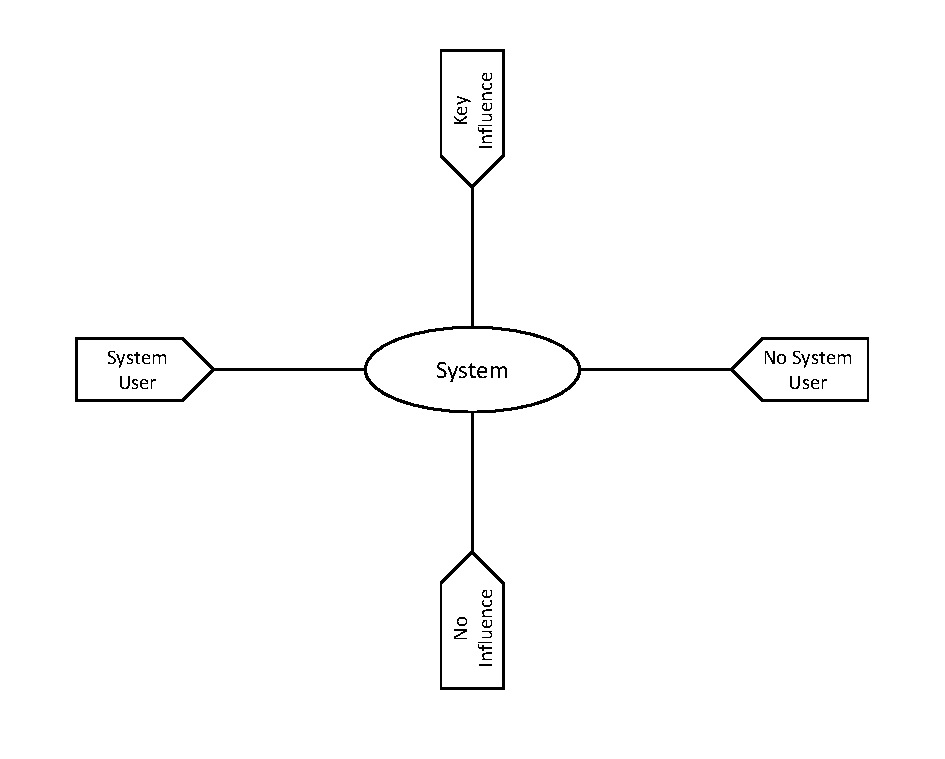
\includegraphics[scale=1]{img/stakeholderMap.pdf}
    \caption[Stakeholder Map]{Stakeholder Map (own illustration based on \cite[38]{Robier.2016})}
    \label{fig:stakeMap}
\end{figure}

\paragraph{} For visualization of relevant stakeholders, \textcite[38]{Robier.2016} suggest the usage of a stakeholder map (cf. \Cref{fig:stakeMap}). People of the left hand side of the vertical axis are the users of the program, divided into heavy users (far left) and fist time users (close to the axis) \parencite[cf.][38]{Robier.2016}. Stakeholders on the right hand side do not use the system, but still influence it \parencite[cf.][38]{Robier.2016}. 

\paragraph{} The vertical axis displays the influence of the stakeholders on the system. A project manager would e.g. be in the upper half, while a service desk employee would be on the bottom half, since he can only make suggestions, but cannot give orders \parencite[cf.][38]{Robier.2016}. 

\paragraph{} This approach does not aim at the identification of each individual stakeholder, but at the identification of stakeholder groups to be represented by a persona \parencite[cf.][82]{Cooper.2007}, explicitly  including non-users \parencite[cf.][84]{Cooper.2007}.

\paragraph{} All traits of a persona should contribute to a bigger picture, and thereby must be intentionally set to suggest intended characteristics \parencite[cf.]{Platt.2016}. Therefore, analysis of the identified personas, includes the specification of traits. 

\paragraph{} As an example: Our persona Kevin Smith (25, male) works at a international bank as foreign trade manager after his studies in financial management at Harvard Business School and needs a way to plan his meetings in accordance to required travel times. In his free time he flies his private single engine plane. If getting asked  whether Kevin needs his schedule in a standardized time zone, such as UTC, the answer will probably be 'yes', because he is on the one hand used to using UTC at work and on the other hand in his hobby. 

\paragraph{} Martha Jones (55, female) works at a local retailer since her diploma from community college, now being store manager, requiring a tool to plan and distribute shifts of her employees. She, on the other hand, will have more use for local time. Martha and Kevin may be personas for a calendar service focused on business customers. 

\paragraph{} All traits of Kevin and Martha will have implications on the conception and development of the hypothetical calendar service. Besides the very different functionality requests of transport service provider integration, respectively shift planning and public calendar provisioning, the age may have implications on the devices used. Also the education implies different kinds of prior knowledge. 

\paragraph{} The prioritization of personas heavily depends on the specific product. It may be done by expected revenue (e.g. for sold services), least specialization (e.g. for training software) or any other reasonable technique for prioritization.

\begin{figure}[H]
    \centering
    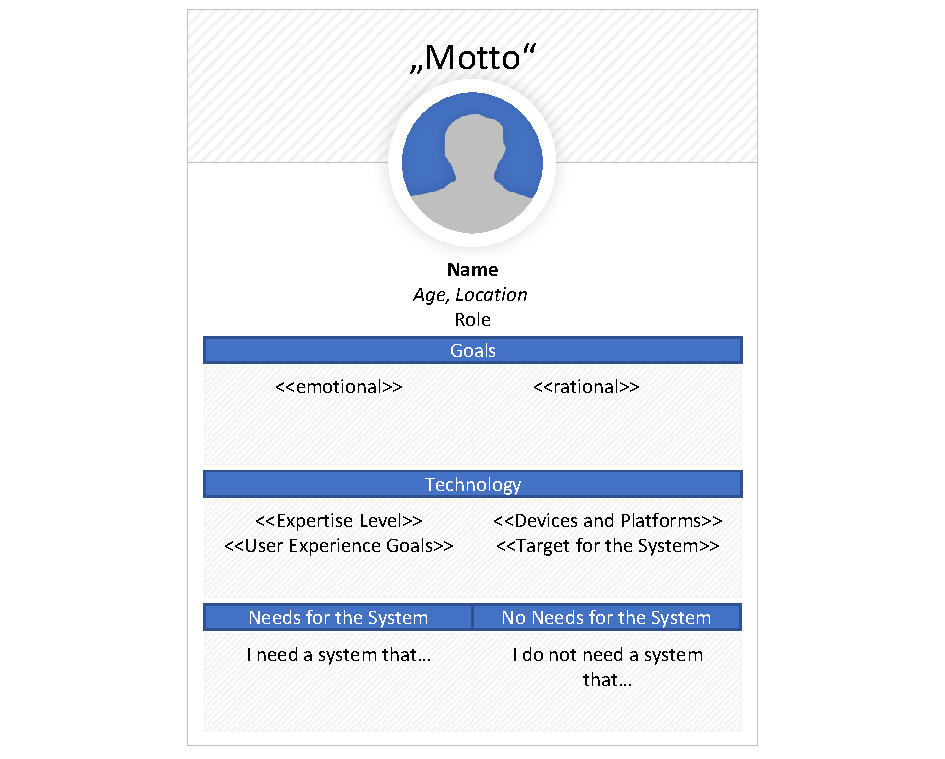
\includegraphics[width=\textwidth]{img/PersonaTemplate.pdf}
    \caption[Template for Personas]{The template used for personas in this paper (own illustration)}
    \label{fig:persTemp}
\end{figure}

\paragraph{} The resulting personas are usually documented in a resume containing all relevant information \parencites[cf.][40]{Robier.2016}[cf.][]{Platt.2016}. This paper will use the template shown in \Cref{fig:persTemp}. It includes a stock photo representing the persona, his or her personal information, his or her goals, needs, and for users his or her technological parameters.


\section{Main Activity}

\subsection{Sourcing Requirements from the Context}

The information of each facet will be compiled into goals for the desired outcome which will then be clustered into the types of requirements described in \cref{ssec:reqTypes} (cf. \Cref{fig:reqTypes} on \cpageref{fig:reqTypes}). The formulation of goals will be done using a sentence stencil and use case diagrams for requirement documentation. 

\paragraph{} The requirements will be itemized and clarified as much as possible to this point. Afterwards, the requirements will be prioritized and potential conflicts will be resolved. The priorities must be clear to know which requirement to drop, in case of an unreasonable conflict.


\subsection{Documenting the Requirements}

\subsubsection{In Natural Language}
Requirements must be expressed distinctly, in order to ensure that the system is correctly developed \parencites[107]{Ebert.2014}. While natural language offers great possibilities, being universaly applicable, flexible and easy to use \parencite[cf.][239]{Pohl.2007}, there are some flaws regarding the distinctiveness. Languages have the troubles of containing  ambiguity, which can be fatal for distinct communication \parencite[cf.][239-243]{Pohl.2007}.

\paragraph{}
\begin{figure}[H]
    \centering
    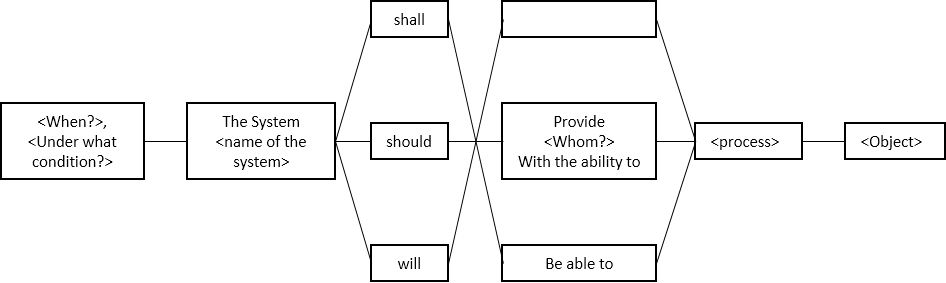
\includegraphics[width=\textwidth]{img/SentenceStructure.png}
    \caption[Requirement Documentation Sentence Structure]{Requirement Documentation Sentence Structure (own illustration based on \cite[246]{Pohl.2007})}
    \label{fig:sentencestructure}
\end{figure}

In order to solve these issues, this paper will use the sentence structure suggested by \textcites[107]{Ebert.2014}[246]{Pohl.2007}. Sentence structures like these help to clarify and structure requirements It is important to note, however, that only one requirement is represented per sentence \parencite[107]{Ebert.2014}. 


\subsubsection{Diagram Notation}
For the diagram documentation of a requirement, a fitting diagram type must be selected \parencite[299]{Pohl.2007}. This thesis will use use models specified in the Unified Modeling Language (UML) 2.5 documentation by the \textcite{ObjectManagementGroup.01.03.2015} with the exception of function diagrams. 


\subsubsection{Use Case Diagram}

\paragraph{\label{par:useCaes}}
Use case diagrams (see below) will be utilized for the documentation of stakeholder's goals. Secondly, this paper will use sequence diagrams, which display the chronological set of interactions, as a tool to visualize scenarios. Last but not least, use cases and scenarios will be merged into function models, which display the flow of information in the complete system and are not part of the UML Specification. 

\begin{figure}[H] 
    \centering
    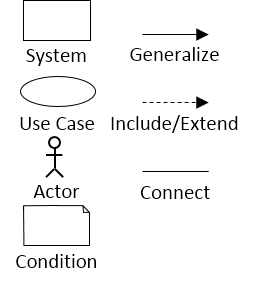
\includegraphics[width=0.28\textwidth]{img/ucSymb.png}
    \caption[Use Case Diagram Notation]{Use Case Diagram Notation (own illustration based on \cite[163]{Pohl.2007}}\label{fig:ucSymb}
\end{figure}

A use case diagram displays goals of stakeholders by abstracting stakeholders into actors, connected to use cases - abstracted goals -, when interacting with the system. Use case diagrams consist of actors, use cases and the system. It display in what kind the actors are directly or indirectly linked to the use cases. Both actors and use cases, can be generalized in an aggregated version of themselves. The notation may be seen in \Cref{fig:ucSymb}.

\begin{figure}[H]
    \centering
    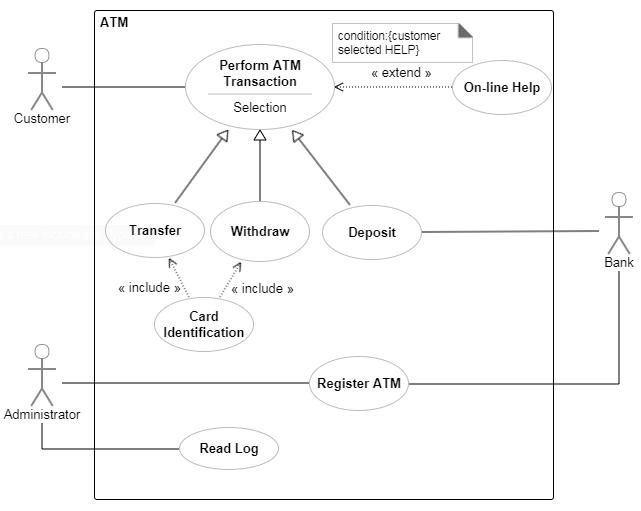
\includegraphics[width=0.73\textwidth]{img/ucEx.png}
    \caption[Use Case Diagram Example]{Use Case Diagram Example (own illustration based on \cite[641-644]{ObjectManagementGroup.01.03.2015})}\label{fig:ucEx}
\end{figure}

\paragraph{} As an example (cf. \Cref{fig:ucEx}): An Automated Teller Machine (ATM) is used by the \ssay{Customer} with the goal \ssay{Perform ATM Transaction}. This can be either \ssay{Transfer}, \ssay{Withdraw}, or \ssay{Deposit} money. For \ssay{Transfer} and \ssay{Withdraw}, a authentication via \ssay{Card Identification} is included. Whenever a use case is included in another, it means that the included use cased must be utilized in order to utilize the including use case \parencite[cf.][639]{ObjectManagementGroup.01.03.2015}. 

\paragraph{} If the \ssay{Customer} requires help \ssay{Perform[ing an] ATM Transaction}, the system offers a \ssay{Selection} with the option \ssay{HELP}. This is regarded as an extension of the goal, as the user does not have to make demands on getting helped \parencite[cf.][638-639]{ObjectManagementGroup.01.03.2015}.

\paragraph{} 
Other actors might have different but also overlapping goals.


\subsubsection{Activity Diagram}

\begin{figure}[H]
    \centering
    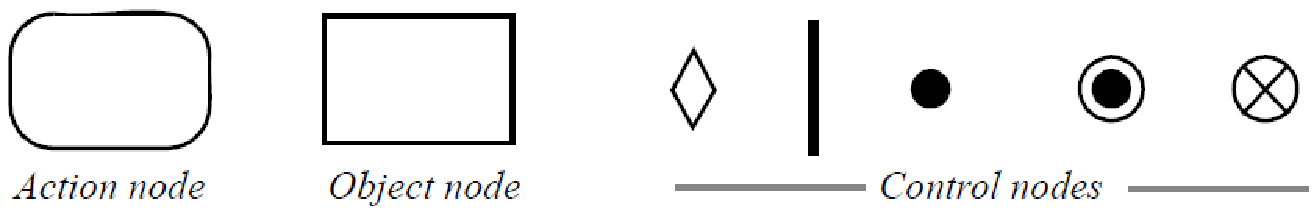
\includegraphics[width=0.7\textwidth]{img/ActivitySymbols.pdf}
    \caption[Activity Diagram Notation]{Activity Diagram Notation \parencite{ObjectManagementGroup.01.03.2015}}\label{fig:adSymb}
\end{figure}

\paragraph{} The activity diagram, on the other hand, expresses a chronological order of activities executed in a use case. These diagrams have a set starting point and at least two end points. In between, actions are connected by control flow lines. This flow can separate and join again to display more complex, non-linear activities  (cf. \Cref{fig:adSymb}).

\begin{figure}[H]
    \centering
    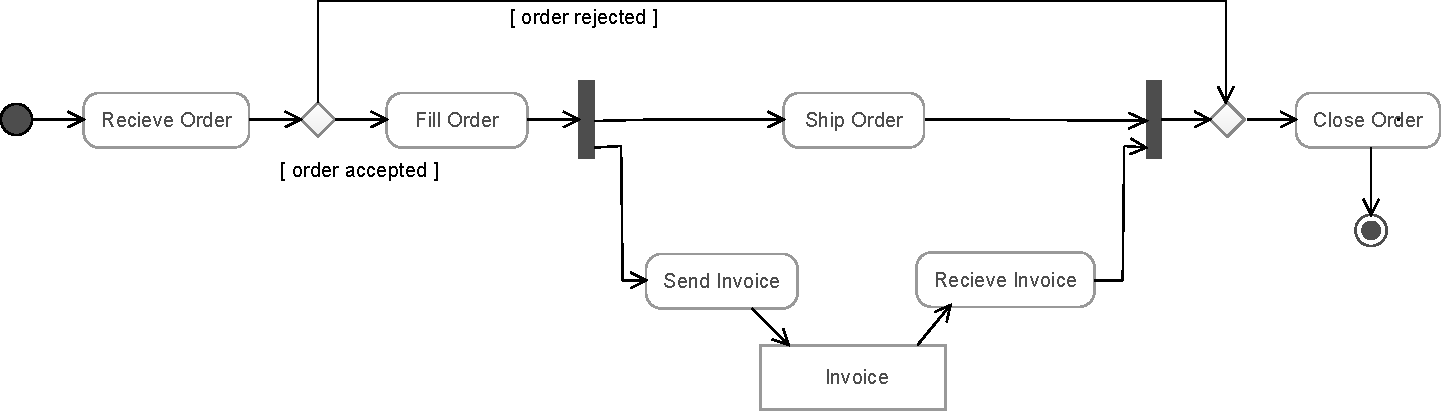
\includegraphics[width=\textwidth]{img/ActivityExample.pdf}
    \caption[Activity Diagram Example]{Activity Diagram Example \parencite[380]{ObjectManagementGroup.01.03.2015}}\label{fig:adEx}
\end{figure}

\paragraph{} For demonstration purposes, \Cref{fig:adEx} shows a order processing activity. After receiving the request, it is decided whether the order is rejected or accepted. If the order is accepted, the order is shipped and an invoice is sent. Once the invoice is received, and the order shipped, the order is closed. \\
In case the order is rejected, it is closed immediately. 

\begin{figure}[H]
    \centering
    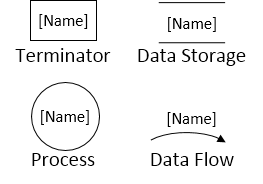
\includegraphics[scale=0.9]{img/fmSymb.png}
    \caption[Function Model Notation]{Function Model Notation (own illustration based on \cite[190]{Pohl.2007})}
    \label{fig:fmSymb}
\end{figure}


\subsubsection{Function Diagram}

As mentioned above, function models will be used for solution oriented requirement modeling. Function models display the flow of data throughout the system from and to each external entity. Those are called \ssay{Terminator[s]} \parencite[190]{Pohl.2007}. Within the system, processes and data storage are nodes of the data flow \parencite[cf.][190-191]{Pohl.2007}. The symbolic representation of those can be seen in \Cref{fig:fmSymb}.  

\begin{figure}[H]
    \centering
    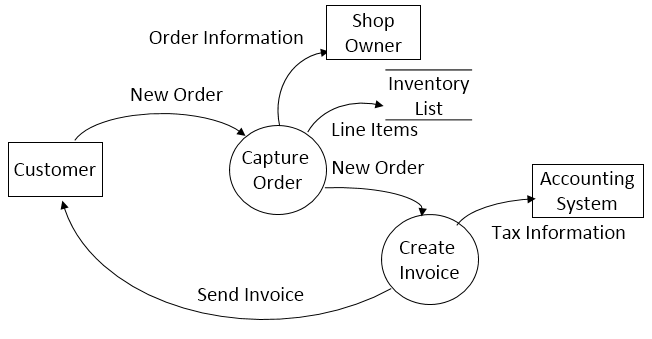
\includegraphics[width=\textwidth]{img/fmEx.png}
    \caption[Function Model Example]{Function Model Example (own illustration)}
    \label{fig:fmEx}
\end{figure}

The example in \Cref{fig:fmEx} illustrates such a function diagram. In this particular example, the system of \Cref{fig.scEx} and \Cref{fig:adEx} is used. Here the customer sends a \ssay{New ORder} to the system, which is processed by \ssay{Capture Order}. This extracts the \ssay{Order Information} and sends those to the \ssay{Shop Owner}. Additionally, the \ssay{Inventory List} is updated and the order is forwarded to \ssay{Create Invoice}, which sends the \ssay{Tax Information} to the \say{Accounting System} and \ssay{Send[s an] Invoice} to the \ssay{Customer}.

\subsection{Conformity}
Whenever conflicts of requirements appear during documentation, or in conception, these will be tried to resolve in cooperation with the stakeholders. 

% \section{Architectural Conception}
% This paper will use UML component diagrams in the alternative notation \parencite[cf.][212]{ObjectManagementGroup.01.03.2015} for architectural composition of the application. An example of a component diagram can be seen in \Cref{fig:comEx}.

% \begin{figure}[H]
%     \centering
%     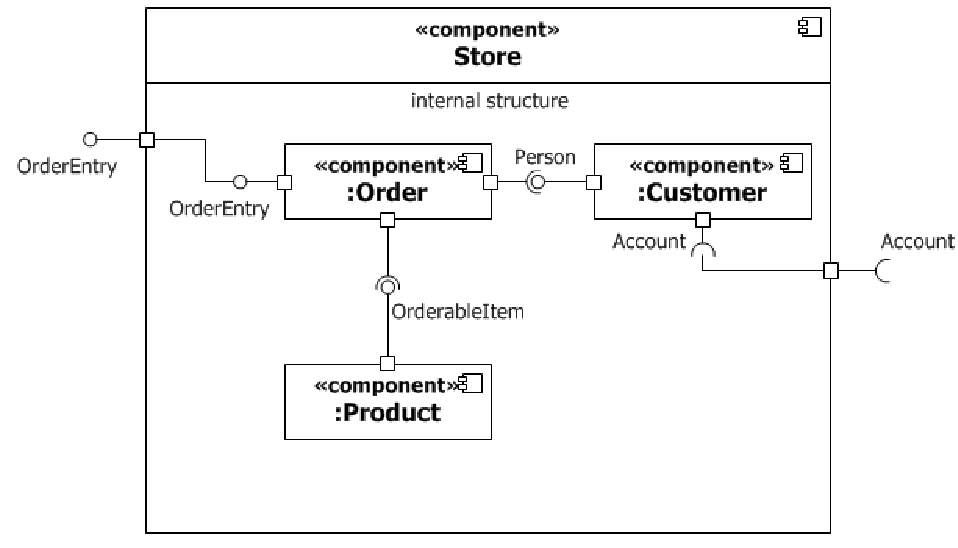
\includegraphics[width=\textwidth]{img/componentExample.pdf}
%     \caption[Component Diagram Example]{Component Diagram Example \parencites[2132]{ObjectManagementGroup.01.03.2015}}
%     \label{fig:comEx}
% \end{figure}

% A component in UML notation may be identified either by the keyword \ssay{<<component>>}, or by a component icon in the top right corner \parencites[cf.][208]{ObjectManagementGroup.01.03.2015}. Both is true for \Cref{fig:comEx}. 

% \paragraph{} In UML structure diagrams, as the component diagram is, entities follow some basic structures:

% \begin{enumerate}
%     \item Entities are labeled by a name, and/or are assigned a  classifier by the \ssay{:[classifier]}-notation  \parencite[cf.][125]{ObjectManagementGroup.01.03.2015}. For instance in \Cref{fig:comEx} \ssay{Store} is the name of a component and its inner components are classified as \ssay{Order},\ssay{Customer}, and \ssay{Product}. If \ssay{Store} gets assigned to a classifier (e.g.~\ssay{Business}), the new label will be \ssay{Store :Business}.
    
%     \item Components can provide and use interfaces, called ports \parencite[cf.][182-184]{ObjectManagementGroup.01.03.2015}. In \Cref{fig:comEx} the component, classified as \ssay{:Product}, provides the interface \ssay{OrderableItem}, which is used by \ssay{:Order}.
    
%     \item Whenever an interface is provided to outside components, a square displays the delegation \parencite[cf.][212]{ObjectManagementGroup.01.03.2015}. In \Cref{fig:comEx} for instance, the port \ssay{OrderEntry} is originally provided by some internal logic of \ssay{:Order}, then delegated to \ssay{Store}, which provides it to other external components. 
% \end{enumerate}


\subsection{User Interface Conception with Wireframes}

Wireframes are early stages of user experience (UX) prototyping \parencite[cf.][]{Rosenzweig.2015}. They will be used in this paper for their simplicity. They are low in fidelity, which is good for testing ideas without exorbitant time and effort \parencite[cf.][]{Platt.2016}. An example can be seen in \Cref{fig:wrEx}

\begin{figure}[H]
    \centering
    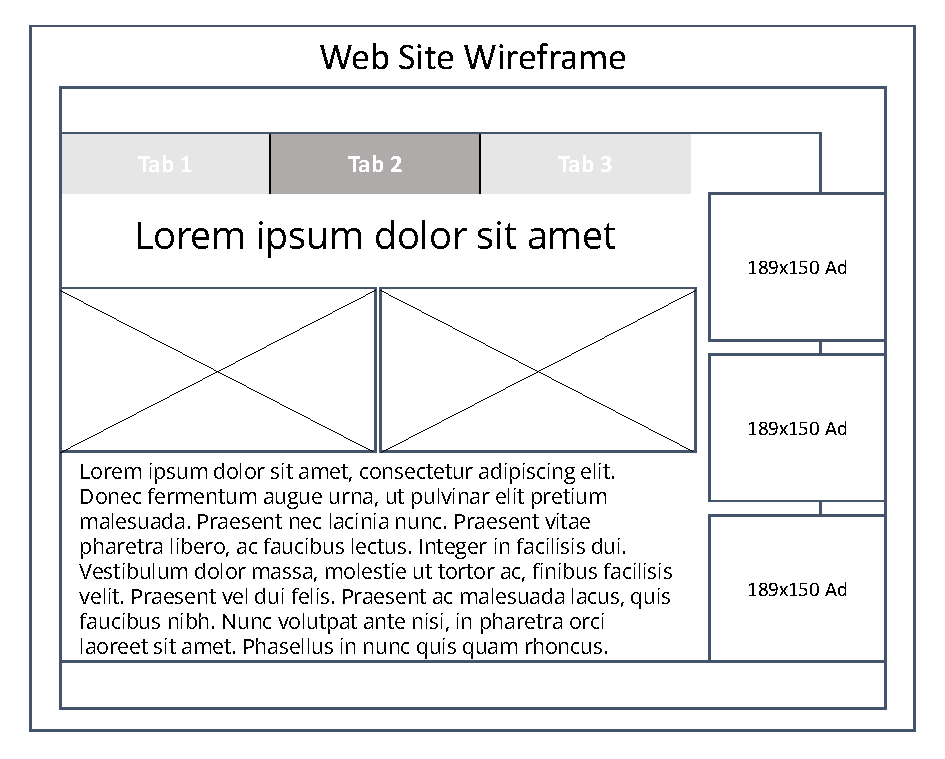
\includegraphics[height=.5\textheight]{img/WireFrameEx.pdf}
    \caption[Wireframe Example]{Wireframe Example (own illustration based on \cite{Rosenzweig.2015})}
    \label{fig:wrEx}
\end{figure}